
\section{Drawings of grammar}
For each accepted word we can associate a graph where the nodes are the
production rule used at that stage to accept the fragment of the string, and
edges are any data needed by that rule to accept the substring.  This is called
the \emph{parse graph}.  In our cases they will always be trees so they are
often called \emph{parse trees}\index{parse tree} but you may also hear them
called \emph{abstract syntax trees} or ``ASTs''.\index{AST}\index{abstract
syntax tree}  In this example $0$ depends on nothing but $S$ depends on an
existing symbol.  Here are the first three parse trees in boxes.
\begin{center}
    \begin{tikzpicture}
    
    \node[draw] (A) at (0,0) {\begin{tikzpicture}
        \node (0) at (0,0) {0};
    \end{tikzpicture}};

    \node[draw] (B) at (3,0) {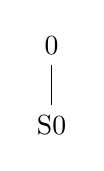
\begin{tikzpicture}
        \node (0) at (0,0) {0};
        \node (S0) at (0,-1) {S0};
        \draw[-] (0) -- (S0);
    \end{tikzpicture}};

    \node[draw] (C) at (6,0) {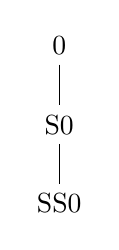
\begin{tikzpicture}
        \node (0) at (0,0) {0};
        \node (S0) at (0,-1) {S0};
        \node (SS0) at (0,-2) {SS0};
        \draw[-] (0) -- (S0);
        \draw[-] (S0) -- (SS0);
    \end{tikzpicture}};
    
    \draw[->] (A) edge["S"] (B);
    \draw[->] (B) edge["S"] (C);
    \draw[dashed,->] (C) edge["S"] (9,0);
\end{tikzpicture}
\end{center}
Between these boxes we have a different graph, the graph that 
plots how one production rule evolves an existing string to another.
This outside graph we call the \emph{word graph}.\index{word graph}  We often condense 
the parse trees to a string to draw the word graph compactly.
\begin{center}
    \begin{tikzpicture}
        \node (0) at (0,0) {0};
        \node (1) at (3,0) {S0};
        \node (2) at (6,0) {SS0};
        \coordinate (3) at (9,0);
        \draw[thick,->] (0) edge["S"] (1);
        \draw[thick,->] (1) edge["S"] (2);
        \draw[dashed,thick,->] (2) edge["S"] (3);
    \end{tikzpicture}
\end{center}

